\documentclass[a3paper, twoside, openany]{book}
\usepackage[utf8]{inputenc}
\usepackage[T1]{fontenc}
\usepackage[italian]{babel}
\usepackage[normalem]{ulem}
\usepackage{textcomp}
\usepackage{array}
\usepackage{amsmath}
\usepackage{amsfonts}
\usepackage{asymptote}
\usepackage{dirtytalk}
\usepackage{gensymb}
%\usepackage{csquotes}
\usepackage{graphicx}
\usepackage{amsthm}
\graphicspath{{assets/}}
\newenvironment{riq}
    {\begin{center}
    \begin{tabular}{|p{0.9\textwidth}|}
    \hline\vspace{0.5pt}}
    { \vspace{5pt}
    \\\hline
    \end{tabular}
    \end{center}
    }
\theoremstyle{definition}
\newtheorem{definition}{Definizione}

\title{Studio dei circuiti RC}
\author{Giacomo Fortunato}

\begin{document}
\maketitle
\section{Presentazione}
Mi chiamo \textbf{Giacomo Fortunato} e frequento (ancora per poco) la quinta classe, sezione F, al Liceo Scientifico Statale \say{G. Battaglini}. Questo è il mio elaborato di \textbf{Matematica e Fisica} preparato per la simulazione del colloquio d'esame (a.s. 2019/2020, anche noto come anno del COVID). \\ In questa breve relazione percorreremo le strade matematiche di integrali e limiti per studiare il funzionamento dei circuiti RC (a corrente continua), in particolare il comportamento del \textbf{condensatore}. \\ Spero che l'elaborato possa essere di Vostro gradimento, buona lettura.
\section{Strumenti utilizzati}
Questo documento è stato creato utilizzando un linguaggio di markup per la preparazione di testi chiamato \LaTeX\footnote{https://www.latex-project.org}: questo linguaggio è utilizzato continuamente nella produzione di documenti, tesi, relazioni e pubblicazioni di ogni genere, particolarmente di carattere scientifico. Personalmente, scrivo e compilo (trasformare da file codice a file finale) \LaTeX con Atom\footnote{https://atom.io}, l'IDE sviluppato da GitHub\footnote{https://github.com}. (Più tecnicamente, utilizzo \textbf{TeX Live 2019} o \textbf{TeX Live 2020}\footnote{https://tug.org/texlive} e, su Atom, utilizzo il pacchetto \textbf{atom-latex} di @thomasjo\footnote{https://github.com/thomasjo/atom-latex}, e il pacchetto \mbox{\textbf{latex-language2e}} di @Aerijo\footnote{https://github.com/Aerijo/language-latex2e}.) \\ Ho appreso di \LaTeX dai miei compagni più grandi delle Olimpiadi di Matematica, e sono fiero di aver imparato così tanto successivamente da solo. \\ Per i diagrammi, ho utilizzato diagrams.net\footnote{https://www.diagrams.net}, un programma javascipt e web-based per la realizzazione di diagrammi. Il software è open-source\footnote{https://github.com/jgraph/drawio} rilasciato sotto Licenza Apache 2.0\footnote{https://github.com/jgraph/drawio/blob/master/LICENSE}.
\chapter{Dimostrazione iniziale}
\section{Introduzione e premesse}
\begin{figure}[htp]
    \centering
    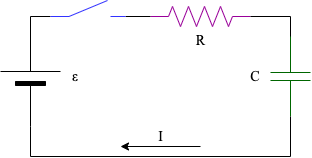
\includegraphics[width=10cm]{Circuito RC-Aperto}
    \caption{Circuito RC aperto}
    \label{fig:RC-aperto}
\end{figure}
Putroppo le condizioni attuali ci impediscono di esplorare troppo a fondo le radici di questo circuito. Tuttavia sarebbe altrettanto sbagliato studiare un circuito RC (figura \ref{fig:RC-aperto}) senza definire poche e semplici definizioni basilari sui circuiti.
\theoremstyle{definition}
\begin{definition}{\textbf{Circuito a corrente continua}}
Un percorso chiuso che viene percorso da una carica, e questa ritorna al suo punto di partenza, è un circuito elettrico a corrente diretta. Sono denominati anche circuiti DC (dall'inglese \emph{Direct Current}).
\end{definition}
\begin{definition}{\textbf{Batteria}}
Una batteria è un dispositivo capace di produrre una differenza di potenziale elettrico ($\Delta V$) ai suoi estremi.
\end{definition}
\begin{definition}{\textbf{Forza elettromotrice indotta, \emph{fem} ($\varepsilon$)}}
La forza elettromotrice indotta è la differenza di potenziale elettrico quando la batteria non genera corrente. Si indica con $\varepsilon$ e si misura in Volt [V].
\end{definition}
\begin{figure}[htp]
    \centering
    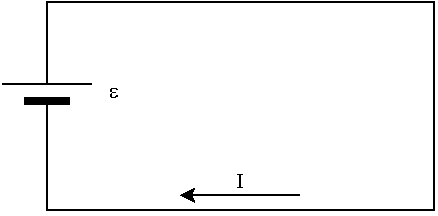
\includegraphics[width=6cm]{Circuito RC-Batteria}
    \caption{Circuito DC con batteria}
    \label{fig:batteria}
\end{figure}
Il filo di un qualunque circuito genera una resistenza al movimento degli elettroni, come se fosse una forma di attrito degli elettroni.
\begin{definition}{\textbf{Resistenza di un filo e prima legge di Ohm}}
La costante di proporzionalità diretta tra la differenza di potenziale $V$ l'intensità di corrente $I$ è la resistenza del filo $R$. Enunciamo quindi la prima legge di Ohm:$$V=IR$$ La resistenza di un filo si misura in Omh $[\Omega]$. Nel modello fisico, se il filo è una linea dritta, la resistenza in quella parte di filo è nulla; per indicare la resistenza in un filo si usa il simoblo in viola nella figura \ref{fig:resistenza}.
\end{definition}
\begin{figure}[htp]
    \centering
    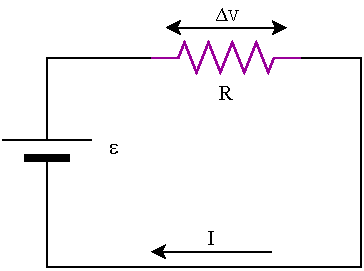
\includegraphics[width=6cm]{Circuito RC-Resistenza}
    \caption{Circuito DC con batteria e resistenza}
    \label{fig:resistenza}
\end{figure}
\begin{definition}{\textbf{Capacità di un condensatore}}
Un condensatore è un dispositivo dotato di due facce piane capaci di accumulare carica elettrica: su una faccia accumula una carica positiva $+q$, sull'altra una carica negativa $-q$ (figura \ref{fig:condensatore-z} e \ref{fig:condensatore-3d}). \\ La carica di un condensatore $Q$ è direttamente proporzionale alla differenza di potenziale $V$, e questo rapporto è la caratteristica del condensatore, la sua capacità. $$C=\frac{Q}{V}$$.
\end{definition}
\begin{figure}[htp]
    \centering
    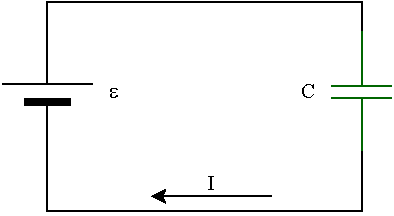
\includegraphics[width=6cm]{Circuito RC-Condensatore}
    \caption{Circuito DC con batteria e condensatore}
    \label{fig:condensatore}
\end{figure}
\begin{figure}[htp]
    \centering
    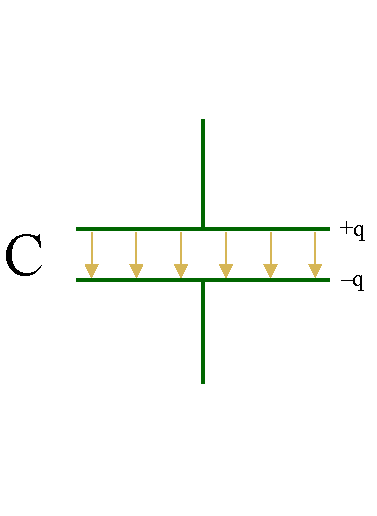
\includegraphics[width=6cm]{Circuito RC-Condensatore-zoom}
    \caption{Ingrandimento del condensatore}
    \label{fig:condensatore-z}
\end{figure}
\begin{figure}[htp]
    \centering
    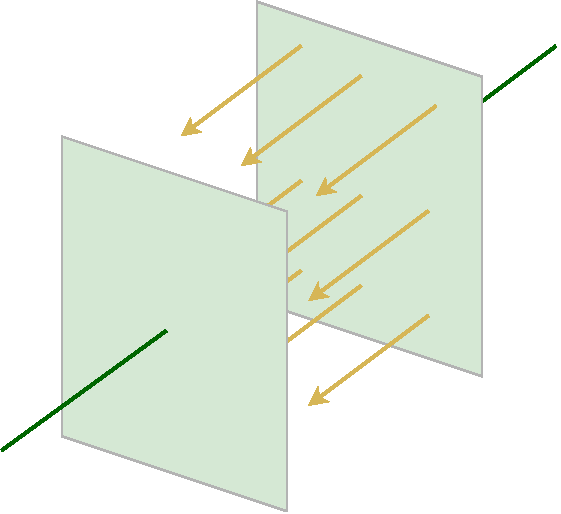
\includegraphics[width=6cm]{Circuito RC-Condensatore-3D}
    \caption{Modello tridimensionale di un condensatore}
    \label{fig:condensatore-3d}
\end{figure}
\begin{definition}{\textbf{Legge dei nodi di Kirchhoff}}
Presupposto che un nodo è un punto del circuito in cui si incontrano 3 o più fili, la somma algebrica di tutte le correnti che convergono in un nodo di un circuito deve essere uguale a 0. Se la corrente esce dal nodo l'intesità sarà di segno negativo, se la corrente entra nel nodo l'intenistà sarà di segno positivo. $$\text{In nodo:}\sum{I_n}=0$$ Nella figura \ref{fig:nodo}, $|I_1+I_2|=|I_3|$, ma in particolare: $$I_1+I_2=-I_3\longrightarrow I_1+I_2+I_3=0$$
\end{definition}
\begin{figure}[htp]
    \centering
    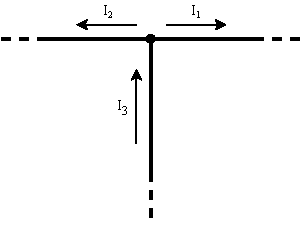
\includegraphics[width=6cm]{Circuito RC-Nodo}
    \caption{Esempio di nodo con intensità di corrente segnate}
    \label{fig:nodo}
\end{figure}
\begin{definition}{\textbf{Legge delle maglie di Kirchhoff}}
Presupposto che una maglia è un qualsiasi segmento di circuito chiuso (compreso tra 2 nodi), la somma algebrica di tutte le differenze di potenziale lungo una maglia di un circuito è uguale a 0. Poiché in ogni circuito dove scorre corrente, è necessariamente presente una batteria, formalizziamo: $$\varepsilon+\sum{\Delta V}=0\longleftrightarrow \varepsilon=-\sum{\Delta V}$$
\end{definition}
\begin{figure}[htp]
    \centering
    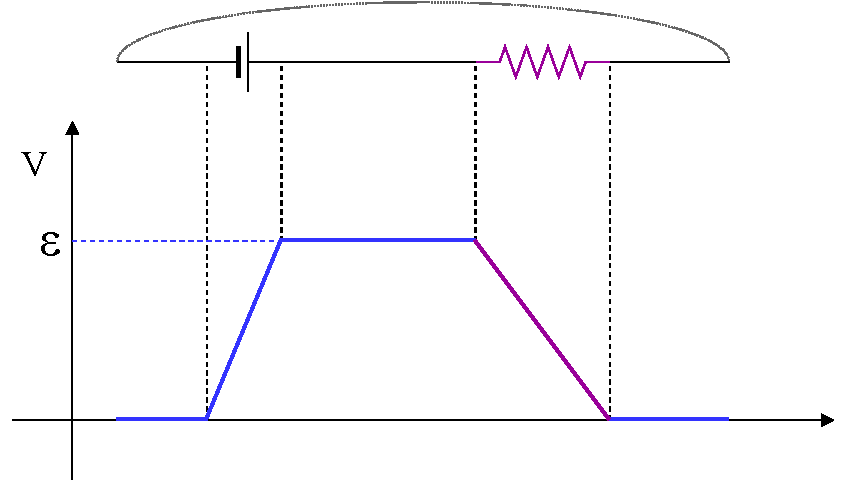
\includegraphics[width=10cm]{Circuito RC-Maglia}
    \caption{Grafico dell'andamento del potenziale in un circuito DC}
    \label{fig:maglia}
\end{figure}
\section{Circuiti RC}













\end{document}
